\documentclass{beamer}
\usepackage{pdfpages}
%Imports and customization
\usepackage{tikz}
\usepackage{graphicx}
\usepackage{tikz-feynman}
\usepackage{ulem}
\usepackage{colortbl}
\graphicspath{ 
    {./images/}
}

\beamertemplatenavigationsymbolsempty
\setbeamertemplate{sidebar right}{}
\setbeamertemplate{footline}{
    \hfill\usebeamertemplate***{navigation symbols}
    \hspace{1cm}\insertframenumber{}/\inserttotalframenumber
}
\setbeamertemplate{caption}{\raggedright\insertcaption\par}
\setbeamersize{text margin left=4mm,text margin right=4mm} 

\setbeamerfont{itemize/enumerate body}{size=\scriptsize}
\setbeamerfont{itemize/enumerate subbody}{size=\scriptsize}
\setbeamerfont{itemize/enumerate subsubbody}{size=\scriptsize}


%Custom Macros
\newcommand{\statwarn}{
    \tiny \color{red} Absolute numbers here mean NOTHING. Plots are based on small (100k events) samples, and are highly biased. All that matters is relative position!
}


% WARNING: When using these commands, the image argument must
% NOT have spaces between itself and the braces
\newcommand{\fullscreenimage}[2]{
    \frame{
        \frametitle{#1} 
        \begin{figure}
        \includegraphics[height=0.9\textheight,width=\textwidth,keepaspectratio]{#2}
        \end{figure}
    }
}


\newcommand{\importpdf}[3]{
    \frame{
        \begin{columns}\column{\dimexpr\paperwidth-10pt}
        \begin{figure}
        \includegraphics[page=#2,height=0.8\textheight,width=\textwidth,keepaspectratio]{#1}
        \end{figure}

        {\tiny #3}
        \end{columns}
    }
}


\newcommand{\displayone}[3]{
    \frame{
        \frametitle{#1} 
        \begin{columns}
            \begin{column}{0.5\textwidth}
                #2
            \end{column}
            \begin{column}{0.5\textwidth}
                \begin{figure}
                    \includegraphics[width=\linewidth,height=\textheight,keepaspectratio]{#3}
                \end{figure}
            \end{column}
        \end{columns}
    }
}

\newcommand{\displayonelarge}[3]{
    \frame{
        \frametitle{#1} 
        \begin{columns}
            \begin{column}{0.3\textwidth}
                #2
            \end{column}
            \begin{column}{0.7\textwidth}
                \begin{figure}
                    \includegraphics[width=\linewidth,height=0.8\textheight,keepaspectratio]{#3}
                \end{figure}
            \end{column}
        \end{columns}
    }
}


\newcommand{\displaytwo}[4]{
    \frame{
        \frametitle{#1} 
        #2
        \begin{columns}
            \begin{column}{0.5\textwidth}
                \begin{figure}
                    \includegraphics[width=\linewidth,height=\textheight,keepaspectratio]{#3}
                \end{figure}
            \end{column}
            \begin{column}{0.5\textwidth}
                \begin{figure}
                    \includegraphics[width=\linewidth,height=\textheight,keepaspectratio]{#4}
                \end{figure}
            \end{column}
        \end{columns}
    }
}

\newcommand{\displaytwocaption}[6]{
    \frame{
        \frametitle{#1} 
        #2
        \begin{columns}
            \begin{column}{0.5\textwidth}
                \begin{figure}
                    \includegraphics[width=\linewidth,height=\textheight,keepaspectratio]{#3}
                    \caption{#4}
                \end{figure}
            \end{column}
            \begin{column}{0.5\textwidth}
                \begin{figure}
                    \includegraphics[width=\linewidth,height=\textheight,keepaspectratio]{#5}
                    \caption{#6}
                \end{figure}
            \end{column}
        \end{columns}
    }
}

\newcommand{\displaytwoVcaption}[6]{
    \frame{
        \begin{columns}
            \begin{column}{0.5\textwidth}
                \frametitle{#1} 
                #2
            \end{column}
            \begin{column}{0.5\textwidth}
                \begin{figure}
                    \includegraphics[width=\linewidth,height=0.3\textheight,keepaspectratio]{#3}
                    \caption{#4}
                \end{figure}

                \begin{figure}
                    \includegraphics[width=\linewidth,height=0.3\textheight,keepaspectratio]{#5}
                    \caption{#6}
                \end{figure}
            \end{column}
        \end{columns}
    }
}


\newcommand{\displaythree}[5]{
    \frame{
        \begin{columns}[T]
            \begin{column}{0.4\textwidth}
                {\usebeamercolor[fg]{title} \insertframetitle{#1} }\\
                \vspace{5mm}
                #2
            \end{column}
            \begin{column}{0.4\textwidth}
                \begin{figure}
                    \includegraphics[width=\linewidth,height=\textheight,keepaspectratio]{#3}
                \end{figure}
            \end{column}
        \end{columns}
        \begin{columns}[T]
            \begin{column}{0.4\textwidth}
                \begin{figure}
                    \includegraphics[width=\linewidth,height=\textheight,keepaspectratio]{#4}
                \end{figure}
            \end{column}
            \begin{column}{0.4\textwidth}
                \begin{figure}
                    \includegraphics[width=\linewidth,height=\textheight,keepaspectratio]{#5}
                \end{figure}
            \end{column}
        \end{columns}
    }
}


\newcommand{\displayfour}[5]{
    \frame{
        \frametitle{#1} 
        \begin{columns}[T]
            \begin{column}{0.4\textwidth}
                \begin{figure}
                    \includegraphics[width=\linewidth,height=\textheight,keepaspectratio]{#2}
                \end{figure}
            \end{column}
            \begin{column}{0.4\textwidth}
                \begin{figure}
                    \includegraphics[width=\linewidth,height=\textheight,keepaspectratio]{#3}
                \end{figure}
            \end{column}
        \end{columns}
        \begin{columns}[T]
            \begin{column}{0.4\textwidth}
                \begin{figure}
                    \includegraphics[width=\linewidth,height=\textheight,keepaspectratio]{#4}
                \end{figure}
            \end{column}
            \begin{column}{0.4\textwidth}
                \begin{figure}
                    \includegraphics[width=\linewidth,height=\textheight,keepaspectratio]{#5}
                \end{figure}
            \end{column}
        \end{columns}
    }
}


\newcommand{\pstrike}[2]{
    \only<-\the\numexpr#1-1>{#2}
    \only<#1->{\sout{#2}}
}


\newcommand{\announcesection}[1]{
    \section{#1}
    \frame{
        \begin{center}
            {\huge #1} 
        \end{center}
    }
}

\newcommand{\kvv}{\kappa_{2V}}
\newcommand{\kl}{\kappa_{\lambda}}
\newcommand{\kv}{\kappa_{V}}

\newcommand{\fkvv}[1]{\kappa_{2V,#1}}
\newcommand{\fkl} [1]{\kappa_{\lambda,#1}}
\newcommand{\fkv} [1]{\kappa_{V,#1}}

\newcommand{\importpdfwpages}[3]{
    \foreach \pageN in {#2,...,#3}{
        \importpdf{#1}{\pageN}{}
    }
}

\newcommand{\hyper}[2]{{\color{blue}\href{#1}{#2}}}



%Begin Presentation
\begin{document}
    \setbeamercolor{background canvas}{bg=}
    \title{Issues in 6-Sample Direct Combination Implementation and Their Effects on Limits }
    \author{Chris Milke}
    \date{19 April, 2021}

    \frame{\titlepage}

    %\frame{\frametitle{Overview} \tableofcontents}

    % Show old limits, explain that many things have needed updating for awhile, and I'm doing that now
    \section{ATLAS Di-Higgs Analysis and MC Sample Combinations}

\displaytwocaption{ATLAS Di-Higgs Analysis}{
    Working with Di-Higgs analysis to discover HH process.
}
{ggF_diagrams}
{$\sigma_{ggF \rightarrow HH}=33.5^{+2.4}_{-2.8}$fb at NNLO}
{vbf-hh_diagrams}
{$\sigma_{VBF \rightarrow HH}=1.73\pm0.04$fb at N\textsuperscript{3}LO}



    % Collection of validation plots, based on mc16d only
    % Sequence of slides showing old basis as it changes with addition of mc16a and then e
    % Show effect mc16e had on limits
    \displaythree{Validation With Only MC16d}
{
    Until now, all my various validation plots were made using only MC16d samples, to simplify implementation.
}
{reco_mHH_cvv0p0cl1p0cv1p0}
{preview_reco_mHH_cvv0p0cl-9p0cv1p0}
{negative_weights_old}


\displaythreeseq{Effect of Other Years on Negative Weights}{
    What does adding different years do to the negative weights?
}{negative_weights_mc16d_old.png}{
    Adding in MC16a reduces negative weights, as expected of more stats
}{negative_weights_mc16ad_old.png}{
    The [0,1,0.5] sample is missing MC16e, and so trying to combine a, d, and e of the 6 samples ruins the linear combination.
}{negative_weights_mc16ade_old.png}

\displaytwocaption{Original 1-D $\kvv$ Limits}
{
    Originally used MC16e in order to be able to compare official 3-term $\kvv$ scan to my 6-term combination.
    
    Other than a lack of fit points close to 1, the two match very well.
}
{c2v_scan_official}
{Official $\kvv$ 3-Term Scan}
{c2v_scan_new_kl1.0}
{6-Term Combination}

\displaytwocaption{Limits without MC16e}
{Attempting to use MC16e in limits caused severe mismodelling of the signal hypothesis}
{2D_scan_2D_scan_test00_samps_vbf_pd_161718_c1v1.0_exclusion}
{Using MC16 a/d/e}
{2D_scan_2D_scan_test01_noMC16e_samps_vbf_pd_1617_c1v1.0_exclusion}
{Using MC16a and MC16d only}


    % Show Nweight integral with integral title
    % Show Top, mid, and current nweights
    % Show result of switching basis on limits
    \frame{
    \frametitle{Finding a Basis with a Better Metric}
        \begin{columns} \begin{column}{0.5\textwidth}
    \begin{center} 
        (70 Possible Combinations of 6... 30 if requiring SM point)

        \resizebox{0.3\textheight}{!}{\begin{tabular}{ |l|l|l| }
            \hline
                \textbf {$\kappa_{2V}$} & \textbf {$\kappa_\lambda$} & \textbf {$\kappa_V$} \\
                \hline
                \rowcolor{red}   0   & 0   & 1   \\ % !!
                0   & 1   & 1   \\ 
                0.5 & 1   & 1   \\ 
                1   & 0   & 1   \\ 
                \rowcolor{red}   1   & 1   & 0.5 \\ % !!
                1   & 1   & 1   \\ 
                \rowcolor{red}   1   & 1   & 1.5 \\ % !!
                1   & 10  & 1   \\ 
                1   & 2   & 1   \\ 
                1.5 & 1   & 1   \\ 
                2   & 1   & 1   \\ 
                4   & 1   & 1   \\ 
                \rowcolor{green} 0   & 1   & 0.5 \\ % !!
                \hline
                \end{tabular}} \end{center}
    \end{column} \begin{column}{0.5\textwidth}
    \begin{center} 
    {\tiny Post-Reco Sample Basis Set}

    \resizebox{0.2\textheight}{!}{ \begin{tabular}{ |l|l|l| }
        \hline
            \textbf {$\kappa_{2V}$} & \textbf {$\kappa_\lambda$} & \textbf {$\kappa_V$} \\
            \hline
            1.  &   1. & 1.  \\
            2.  &   1. & 1.  \\
            1.5 &   1. & 1.  \\
            0.  &   1. & 0.5 \\
            1.  &   0. & 1.  \\
            1.  &  10. & 1.  \\
            \hline
            \end{tabular}}
    \end{center}

    \begin{figure}
    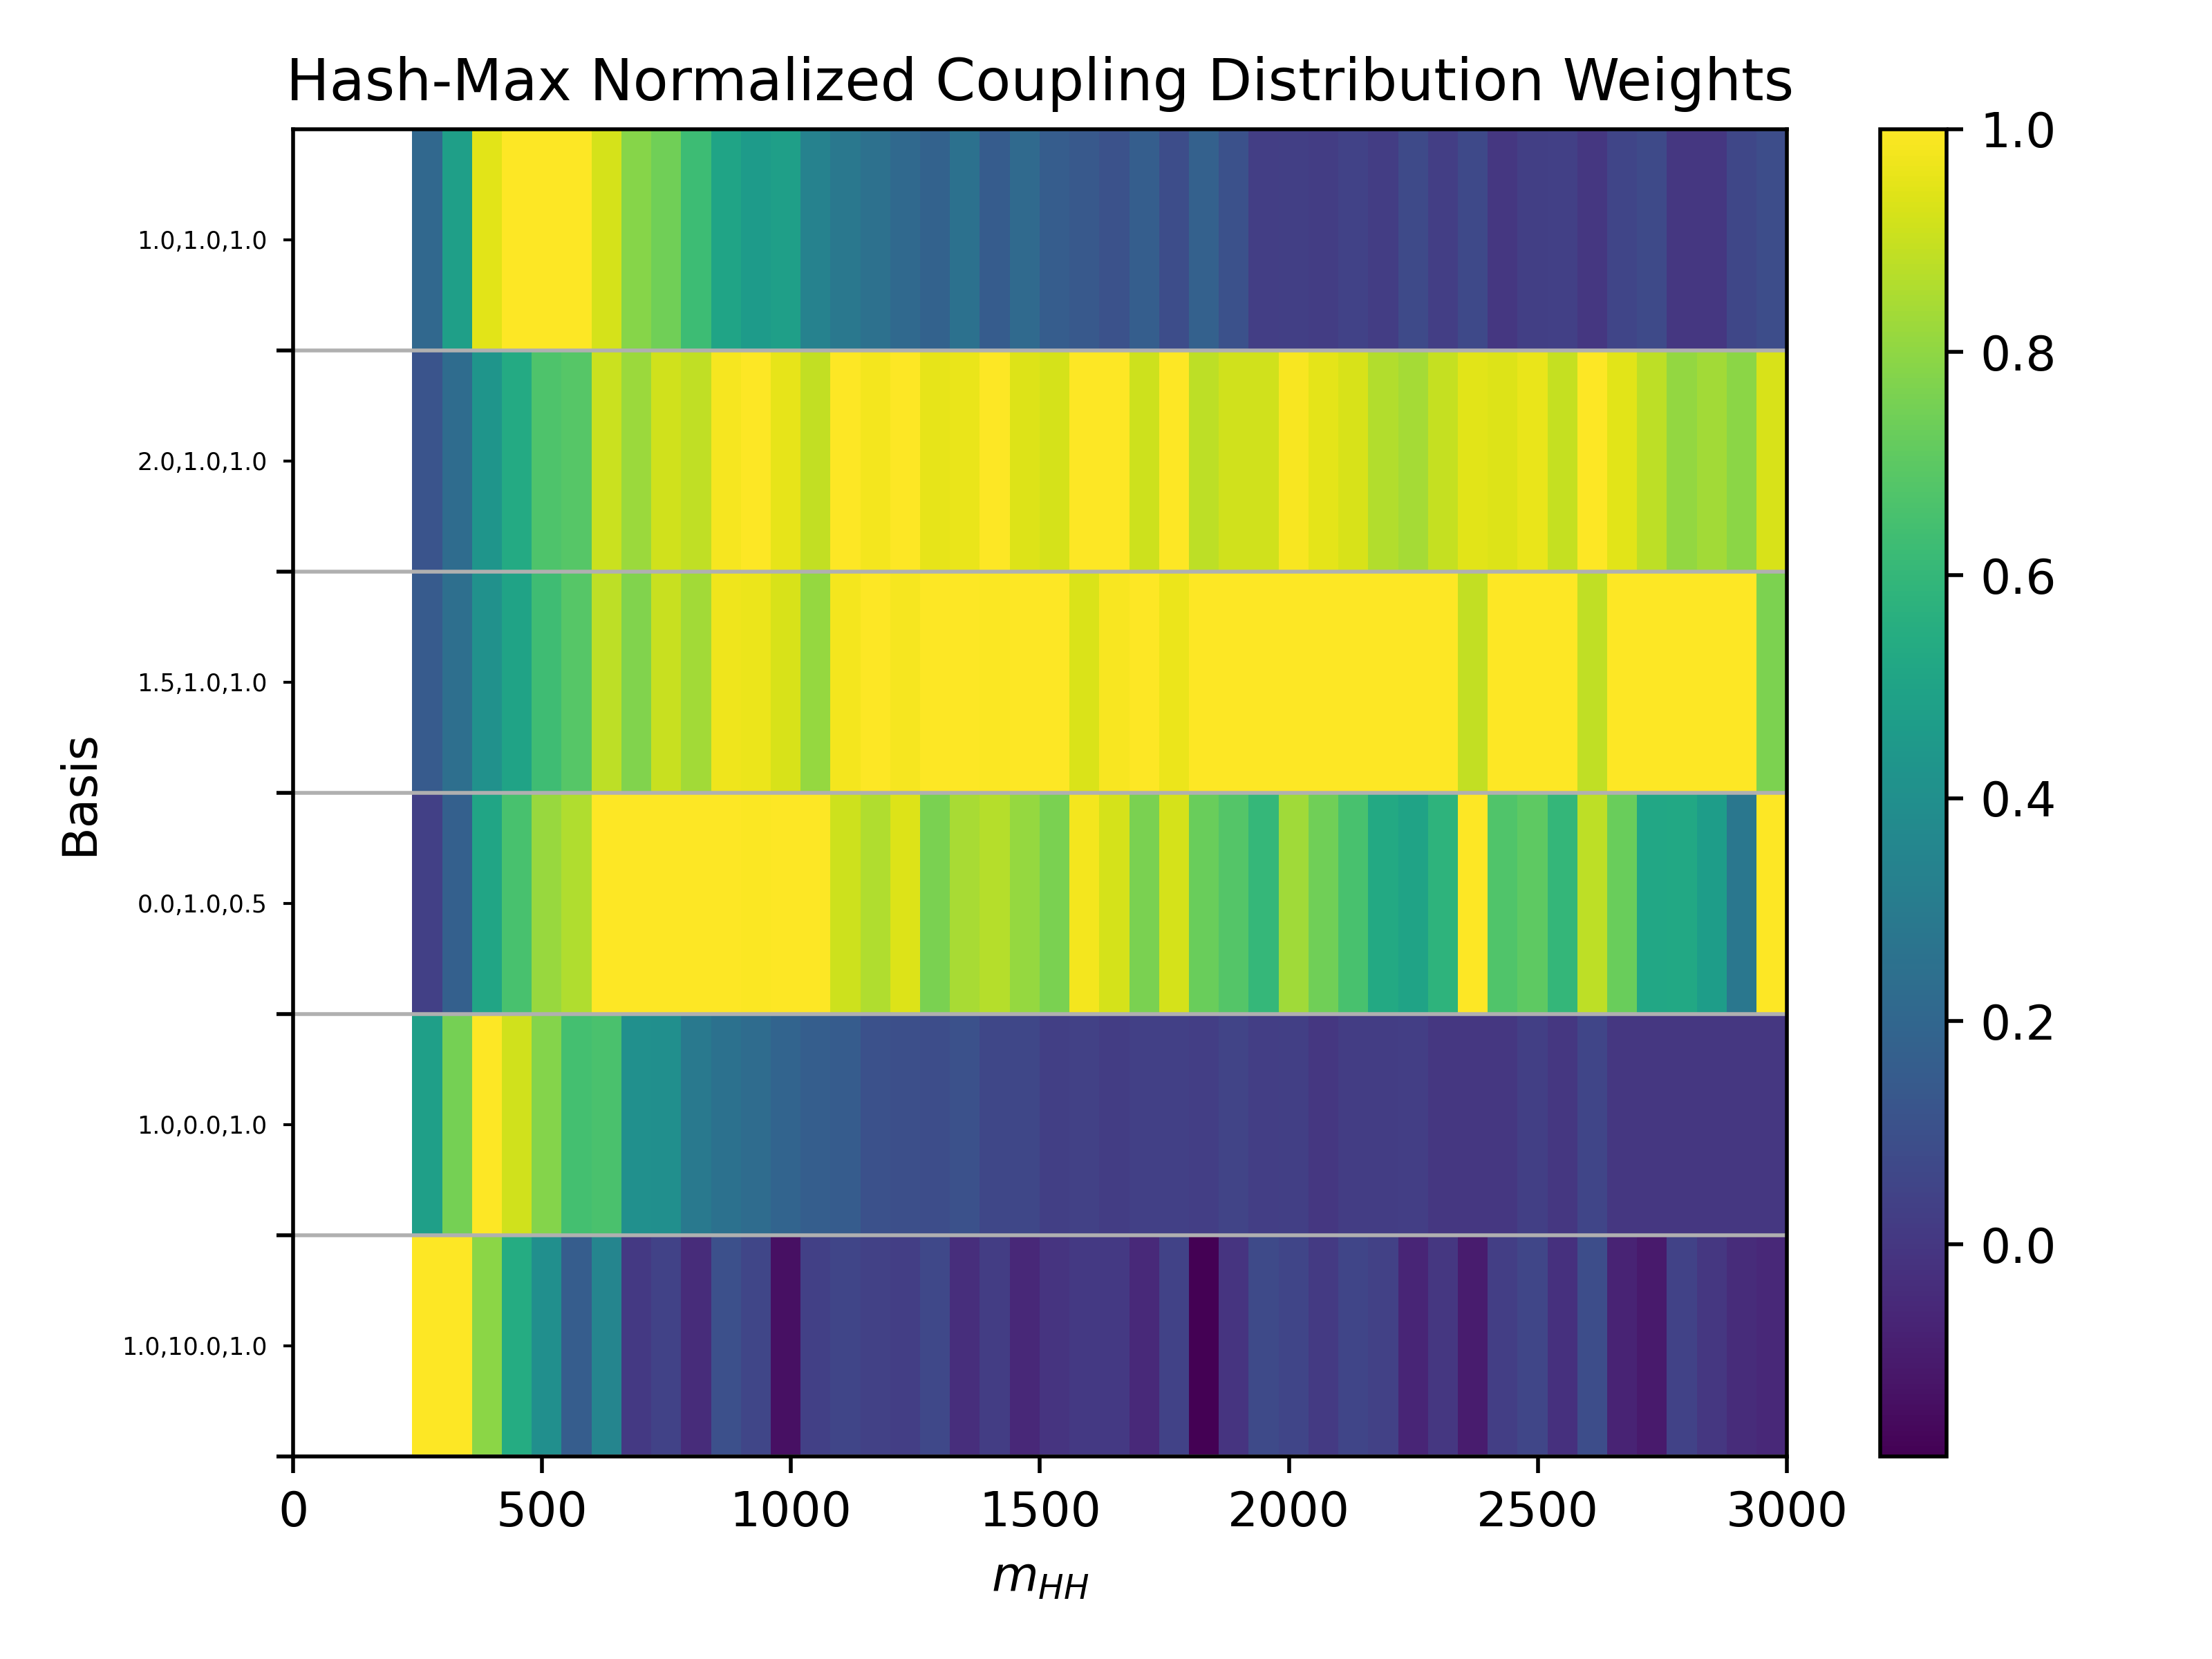
\includegraphics[width=\linewidth,height=\textheight,keepaspectratio]{coupling_scan_auto_chosen_reco_R0_hash_max}
    \end{figure}
    \end{column} \end{columns}
}

\displayonelarge{Ranking Basis by Negative Weight Integral}{
    Take the surface integral of the number of negative bins at each point at in the $\kappa$ parameter space (mutliplying by the $\kvv \times \kl$ ``area" of each square)
}{negative_weights_rank027}

\displaythree{Negative-Weight Map of Different Bases}{
    Other bases show considerable improvement in the number of negative bins
}
{negative_weights_rank027}
{negative_weights_rank015}
{negative_weights_rank000}


\displaytwocaption{Limits with Negative-Weight Integral Rank-1 Basis}{
    Fewer negative weights results in a much more ``natural" limit boundary.

    Sharp edges and corners appear to have been a consequence of poor signal modelling.
}
{2D_scan_2D_scan_test01_noMC16e_samps_vbf_pd_1617_c1v1.0_exclusion}
{Using old basis}
{2D_scan_2D_scan_test02_newBasis_samps_vbf_pd_1617_c1v1.0_exclusion}
{Using new basis}


    % Show progression of limits (old -> noMC16e -> new basis)
    \displaythreecaption{Limit Change Overall}{
        Overall affect of changes has completely altered the shape of the 2D limits.
    }
    {2D_scan_2D_scan_test00_samps_vbf_pd_161718_c1v1.0_exclusion}
    {Old basis with MC16e}
    {2D_scan_2D_scan_test01_noMC16e_samps_vbf_pd_1617_c1v1.0_exclusion}
    {Old basis, NO MC16e}
    {2D_scan_2D_scan_test02_newBasis_samps_vbf_pd_1617_c1v1.0_exclusion}
    {New basis, NO MC16e}


    %Conclusion; Mention that systematics *still* don't work for some reasons...
    \frame{
        \frametitle{Conclusion}
        \begin{itemize} {
            \item Missing MC16e sample had a much larger impact than anticipated
            \item New basis optimization metric reveals poor performance of old basis
            \item New limit shape after correcting for these is very different
            \item Limits \textit{still} do not include bgd systematics (working on this now)
            \item Will continue checking to see if any other issues of this nature exist
        } \end{itemize}
    }

    %\announcesection{Backup}

\end{document}
